\chapter{Methodology}
\label{chapter:chapter03}

This chapter explains the different parts of the problem and the strategies to solve it. Section~\ref{sec:Problem_design} describes how the problem is structured, the size of the search space, and how a feasible solution looks like. Then, in Section~\ref{section:objective_functions} details the objective functions are described, as well as a justification of why each of them was chosen. Finally, Section~\ref{sec:operators} defines the operators to be used by the optimisation algorithms and the reasoning behind them.\\

\section{Problem Design} \label{sec:Problem_design}

The problem established is described as given a data set $D$ of $n$ students, $D = (s_1,...,s_n)$, a solution $A$ consists of an optimal arrangement of groups $G$, which assigns each student to a group, $A = \langle s_i \leftarrow G_j, \ldots, s_n \leftarrow G_m \rangle$, with the students being in the same group optimising their preference criteria as described in Section~\ref{section:preference_criteria}. Thus, the optimisation encompasses the following goals:

\begin{itemize}
    \item Finding the less distance between the level of experience of the students inside the same group.
    \item Finding the less distance among an ontology of interests, where similar interests related interests are in the same branch.
    \item Having a group size near the ideal group size which is arbitrarily defined as between four and five.
    \item The percentage of participation which is how much the students participate in the conversation of the group, maximising for the most participation.
\end{itemize}

The solution is then the group number for each student, which serves as identification. The solution should ensure maintaining the preference of the user within the group, regardless of the order in which the groups are presented. This can be seen in Figure~\ref{fig:dataset_eg} and Equation~(\ref{eq:students_groups}).\\

\begin{equation}
  \label{eq:students_groups}
  \begin{gathered}
        D = (s_0,s_1,s_2,s_3,s_4,s_5,s_6,s_7,s_9,...,s_n),\\
        A = \langle s_0 \leftarrow G_3, s_1 \leftarrow G_0, s_2 \leftarrow G_2,     s_3 \leftarrow G_1, s_4 \leftarrow G_3, s_5 \leftarrow G_1,...  \rangle
  \end{gathered}
\end{equation}


There are two manners to approach the problem. The first one considers the groups as the variables and the students as the values, while the second one considers the students as the variables and the groups as the values. The second approach, however, has the disadvantage that the number of variables becomes inconsistent depending on the size of the groups. Another disadvantage is that some groups could remain empty, and the crossover and mutation added unnecessary complexity to the task. The former approach does not present these disadvantages and is the chosen one to use.\\

A linked list is further kept to internally track the groups and make easy the evaluation of objective functions, which means if $s_i \leftarrow G_j$ then $G_j = (...,s_i,...)$.\\

%REWRITE

The search space comprehends all the possible assignments of groups to the students. This is related to the Bell number, which counts the possible partitions of a set. The Bell number is defined recursively as:

\begin{equation}
    B_{n+1} = \sum_{k=0}^n \binom{n}{k}  B_k
\end{equation}

\noindet where $B_k$ is the number of partitions for a set with $k$ elements.\\

The neighbourhood is composed of every solution that has a single student in a different group, among the feasible solutions.\\

Figure~\ref{fig:dataset_eg} presents a sample of a dataset with each of its different features, as it can be seen the Group $G_3$ is assigned to students according to the preference criteria.\\

\begin{figure*}[!htp]
    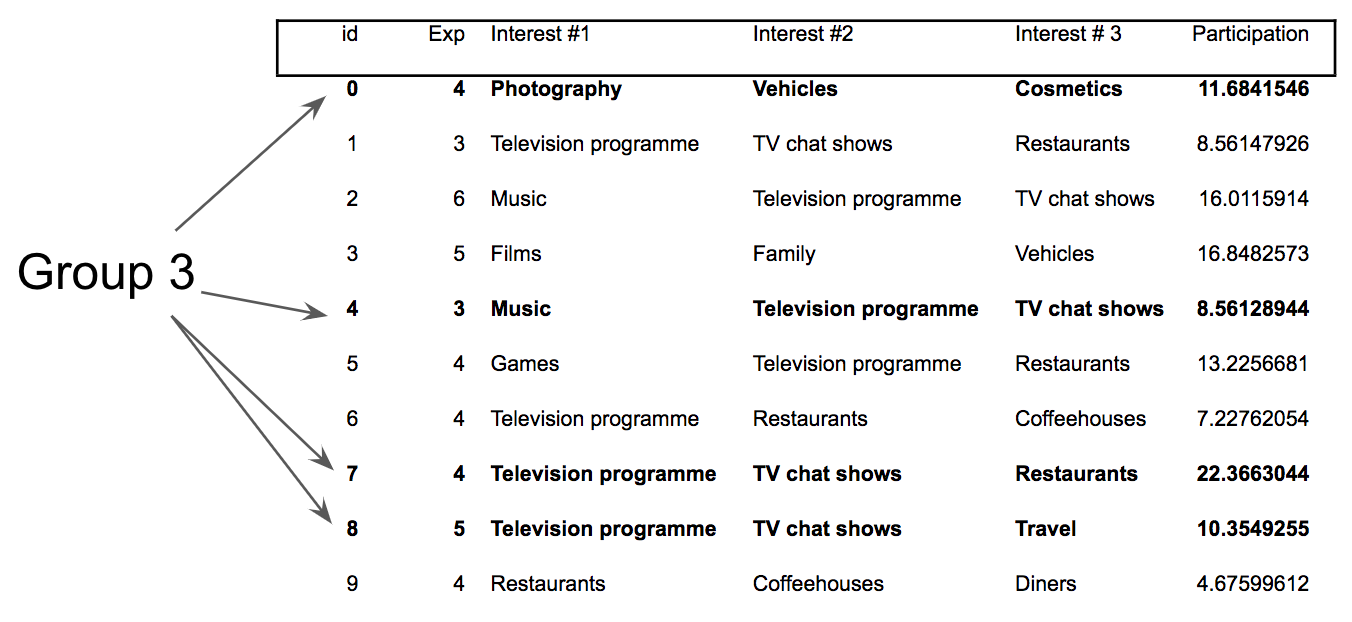
\includegraphics[width=0.85\textwidth]{images/dataset_eg.png}
    \caption{This is an example of a data set of nine users, each with their experience, three different interests and a participation percentage.}
    \label{fig:dataset_eg}
\end{figure*}

\section{Objective Functions} 
\label{section:objective_functions}

In the following section, the different objective functions are described, which are based on the preference criteria defined in Section~\ref{section:preference_criteria}, the experience level, the interests similarity, and the participation style. It should be noted that preference criteria are evaluated per group $G$. Then, the objective values for a solution $A$ are computed as the average of each preference criterion. For instance, for the Group Size~$Gs(A) = AVG(Gs(G_i),...,Gs(G_n))$.\\

\subsection{Group Size}
\label{subsection:group_size}

For this research, the ideal group size $Gs$ is arbitrarily considered from four to five students. This size is based on the idea that it will allow users belonging to the same group to participate homogeneously. It is also possible that there might be groups with $gs_{min} = 3$ or $gs_{max} = 6$ students, but these are not considered as ideal group sizes. Nonetheless, these non-ideal groups sizes are still considered as feasible group sizes, so that other features, such as the \textit{participation style} or the \textit{interests similarity} results in a better cohesion of the group.\\

The corresponding objective function measures the distance to $4.5$ since four and five are considered equally ideal and $4.5$ is just the average between both. Thus, the objective function is defined as:

\begin{equation} \label{eq_group_size}
    Gs(G_i) = | Gs(G_i) - 4.5 |
\end{equation}

\subsection{Experience level}
\label{subsection:experience_level}

The experience level $Lvl$ in the language is taken from the standard \textbf{CEFR}. The values considered for each level are A1, A2, B1, B2, C1 y C2, which are sorted from the most basic to the most advanced level. Therefore, a numeric value is assigned to each of them from zero to five, where zero corresponds to A1 and five corresponds to C2. The intention for assembling the groups is that the users inside them do not have much variation in their experience level. 
In this way, the vocabulary used is not too advanced for the lower student levels or too simple for more advanced users. 

Equation~(\ref{eq_nivel}) calculates the standard deviation $\sigma$ of the level of each student is considered. An ideal group should have a standard deviation of zero, indicating that all users from a group have the same experience level.\\

\begin{equation} \label{eq_nivel}
    Lvl(G) = \sqrt{\frac{1}{Gs(G)-1} \sum_{i=1}^{Gs(G)} (Lvl(s_i) - \overline{Lvl(s)})^2}
\end{equation}

where $Gs(A)$ is the size of the group, $Lvl(s_i)$ is the level of a particular user and $\overline{Lvl(s)}$ is the average of the level of all the users in the group.

\subsection{Interests Similarity}
\label{subsection:interests_similarity}

To calculate the interests similarity $Int$, a strategy similar to the one described in~\cite{taxonomy_semantic_similarity} is used. All the interests are considered a vector of values, where each of them is ranked based on the distance it takes to reach each other interest in the ontology defined by the Social Network Facebook. Each interest has assigned a value of $d_i$, which indicates this distance. It represents how related is a particular interest related to others. For example, if the ontology is seen in Figure~\ref{fig:facebook_ontology} is taken into account, the interest "Graphic Design" is a branch of "Design" which in turn is a branch of "Business and Industry", therefore it would have a value of two with respect to "Business and Industry", a value of one with respect to "Design" and a value of zero for itself. \\

\begin{figure}
    \centering
    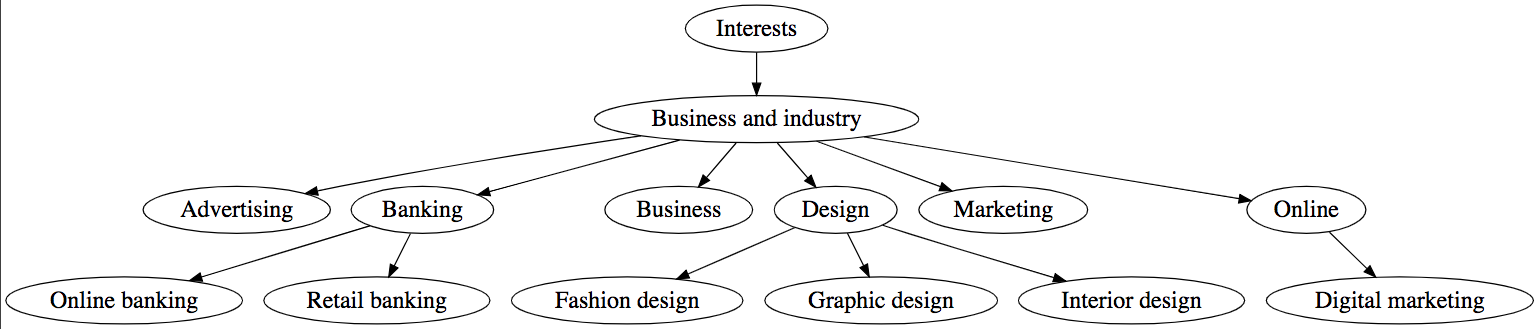
\includegraphics[width=150mm]{ontology.png}
    \caption {An example of the Facebook interests ontology.}
    \label{fig:facebook_ontology}
\end{figure}

These values are then normalised by a factor of $1/(1+d)$. The interest vector for a user is confirmed by the maximum value of this normalisation. 
For example, a student $s_a$, with "Graphic Design", "Interior Design", and "Banking" as his/her interest, has an interest vector equals to $Ints(s_a) = \langle Business \gets 0.50, Design \gets 0.50, Graphic Design \gets 1.00,...\rangle$ and a student $s_b$, with "Retail Banking", "Advertising", and "Running" as his/her interest, has an interest vector equals to $Ints(s_b) = \langle Business \gets 0.33, Advertising \gets 0.50, Banking \gets 0.50,...\rangle$. The complete process can be seen in Table~\ref{tab:interests_s_1} for the student $s_a$ and in Table~\ref{tab:interests_s_2} for the student $s_b$.\\

\begin{table}[]
\centering
\resizebox{\textwidth}{!}{
\begin{tabular}{ccccccc}
\hline
                & Interests & Business & Design   & Graphic Design & Interior Design & Banking  \\ \hline
Graphic Design  & 3         & 2                     & 1        & 0              & $\infty$        & $\infty$ \\ 
Interior Design & 3         & 2                     & 1        & $\infty$       & 0               & $\infty$ \\ 
Banking         & 2         & 1                     & $\infty$ & $\infty$       & $\infty$        & 0        \\ 
                &           &                       &          &                &                 &          \\  
Graphic Design  & 0.25      & 0.33                  & 0.50      & 1.00              & 0.00               & 0.00        \\ 
Interior Design & 0.25      & 0.33                  & 0.50      & 0.00              & 1.00               & 0.00        \\ 
Banking         & 0.33      & 0.50                  & 0.00      & 0.00              & 0.00               & 1.00        \\ \hline
\end{tabular}
}
\caption{Interests mapping of a $s_1$ example user.}
\label{tab:interests_s_1}
\end{table}


\begin{table}[]
\centering
    \resizebox{\textwidth}{!}{
        \begin{tabular}{cccccccc}
        \hline
                        & Interests & Business & Advertising & Banking  & Retail Banking & Hobbies  & Running  \\ \hline
        Retail Banking  & 3         & 2        & $\infty$    & 1        & 0              & $\infty$ & $\infty$ \\ 
        Advertising & 2         & 1        & 1           & $\infty$ & $\infty$       & $\infty$ & $\infty$ \\ 
        Running         & 3         & $\infty$ & $\infty$    & $\infty$ & $\infty$       & 1        & 0        \\ 
                        &           &          &             &          &                &          &          \\ 
        Retail Banking  & 0.25      & 0.33 & 0.00          & 0.50      & 1.00              & 0.00        & 0.00        \\ 
        Advertising & 0.33  & 0.50      & 0.50         & 0.00        & 0.00              & 0.00        & 0.00        \\ 
        Running         & 0.25      & 0.00        & 0.00           & 0.00        & 0.00              & 0.50      & 1.00        \\ \hline
        \end{tabular}
    }
    \caption{Interests mapping of a $s_2$ example user.}
    \label{tab:interests_s_2}
\end{table}

\begin{table}[]
\centering
\resizebox{\textwidth}{!}{
    \begin{tabular}{cccccccccc}
    \hline
          & Interests & Business & Design & Graphic Design & Interior Design & Banking & Retail Banking & Hobbies & Running \\ \hline
    $Ints(s_a)$ & 0.75      & 0.5      & 0.5    & 1              & 1               & 1       & 0              & 0       & 0       \\
    $Ints(s_b)$ & 0.33      & 0.5      & 0      & 0              & 0               & 0.5     & 1              & 0.5     & 1       \\ \hline
    \end{tabular}
}
\caption{Comparison of interests between $s_a$ and $s_b$.}
\label{tab:interests_comparison}
\end{table}

To compare the interests of a student to another student, the cosine $cos(\theta)$ distance, shown in Equation~(\ref{eq:cos_sym}), is used. When the users have identical interests, their cosine distance becomes one, and zero for completely different interests. Since we are minimising, the objective function is considered as $f = 1 - f_{int}$. An example of two interests vectors of two users can be seen in Table~\ref{tab:interests_comparison}, here $1 - f_{int}(s_a,s_b) = 0.29$ which is considerably similar because both students share interests such as: \\

\begin{equation} \label{eq:cos_sym}
     f_{int}(s_a,s_b) = \frac{ \sum\limits_{i=1}^{n_{int}}{Int(s_a)  Int(s_b)} }{ \sqrt{\sum\limits_{i=1}^{n_{int}}{Int(s_a)^2}}  \sqrt{\sum\limits_{i=1}^{n_{int}}{Int(s_b)^2}} }   
\end{equation}

\noindent where $Int(s_a)$ is the interest vector of a user and $Int(s_b)$ is the interest vector of another and $n_{int}$ is the number of Interest of $s_a$ and $s_b$ combined.\\

The similarity of interests of a group $G$ is the average of all the interests function $f_{int}(s_a,s_b)$ for all the students in the group.\\

\subsection{Participation style}

%It was a difficult task to find a defined function that calculated the participation in a group or a special configuration of participation styles that promoted the participation of all students.

There is no defined function that allows calculating participation of $Ps$ in a group or a special configuration of participation styles, which promotes the participation of all students. 
However, as mentioned in Section~\ref{section:functional_roles}, we make use of Benne and Sheats functional roles~\cite{FunctionalRoles}. One particular role is defined as \textit{protagonist}, which is a role that implies participation. A member in a group does not have a particular role defined, but they may have different roles as the conversation goes on. Therefore, a percentage of \textit{protagonism} can be defined for each student representing how much was the role \textit{protagonist} present in a conversation.\\

Since it is desired to have high participation in a group, and the problem is minimisation, then the participation style is considered as the inverse of the sum of all the participation percentage of protagonism of the students of a group, this is simply defined in Equation~(\ref{eq:particiPation}).\\

\begin{equation}
    \label{eq:particiPation}
    Ps(G_i) = \frac{1}{\sum P(s_i)} 
\end{equation}

Where $Ps(s_i)$ is the percentage of protagonism of each of the students of the group. \\

\section{Stability}
\label{section:stability}

Stable Student Groups are described as:

\begin{definition}
    For a Solution, $A$ is considered stable if and only if there is no student from any group $G_a$ that would prefer to belong to another group $G_b$, i.e., students are satisfied with the group that they belong to.
\end{definition}

The reason a student $s_a$ may want to leave their group for another is that they perceive a considerable gain from doing the switch. For example, the students from $G_b$ might have more common interests with $s_a$. This preference is defined by the factors from the preference criteria, the interests similarity, the level similarity, their participation style compared to the other students from their group and the group size.\\

Taking this into account, the satisfaction according to their preference is calculated using the same objective functions defined earlier. Once the groups are made, the evaluation of each of the objective functions is assigned from each student towards the rest of the members of the group, and the other groups. "How much they would like to belong to any other group?"\\

Suppose we have the following data-set $D$:\\

\begin{table}[H]
\centering
\resizebox{\textwidth}{!}{
\begin{tabular}{ccccccc}
\hline
id & Level & Interest 1 & Interest 2 & Interest 3 & Participation percentage \\
\hline
0   &    4   &    Photography            &    Vehicles   &    Cosmetics                    &    11.68 \\
1   &    3   &    Television programme   &    TV chat shows   &    Restaurants             &    8.56  \\
2   &    6   &    Music                  &    Television programme   &    TV chat shows    &    16.01 \\
3   &    5   &    Films                  &    Family   &    Vehicles                       &    16.84 \\
4   &    3   &    Music                  &    Television programme   &    TV chat shows    &    8.56  \\
5   &    4   &    Games                  &    Television programme   &    Restaurants      &    13.22 \\
6   &    4   &    Television programme   &    Restaurants   &    Coffeehouses              &    7.22  \\
7   &    4   &    Television programme   &    TV chat shows             &    Restaurants   &    22.36 \\
8   &    5   &    Television programme   &    TV chat shows             &    Travel        &    10.35 \\
9   &    4   &    Restaurants            &    Coffeehouses              &    Diners        &    4.67  \\
\hline
\end{tabular}
}
\caption{Example dataset of 10 students}
\label{tab:example_dataset}
\end{table}

Let's assume we find the solution: $ A = \langle G_0 \leftarrow (s_0,s_1,s_2,s_4,s_5), G_1 \leftarrow (s_3,s_6,s_7,s_8,s_9) \rangle$, for this example we make use of the Interests Similarity function alone. In Table~\ref{tab:int_stability} the Interest Similarity is calculated from each user towards every other from the data-set. Then, the average of these values is calculated, this value represents "How much they would like to leave their group for the other?" according to the rest of the members. After that, the same is done for the other groups, representing "How much they would like to leave this group if they were a member?".\\

% Please add the following required packages to your document preamble:
% \usepackage{graphicx}
% \usepackage[table,xcdraw]{xcolor}
% If you use beamer only pass "xcolor=table" option, i.e. \documentclass[xcolor=table]{beamer}
\begin{table}[H]
\centering
\resizebox{\textwidth}{!}{%
\begin{tabular}{cccccccccccccc}
\hline
Student & $s_3$ & $s_6$ & $s_7$ & $s_8$ & $s_9$ &  & $s_0$ & $s_1$ & $s_2$ & $s_4$ & $s_5$ &  & Stable? \\
\hline
$s_3$ & 1.00 & 0.05 & 0.05 & 0.58 & 0.02 & \cellcolor[HTML]{C0C0C0}{\color[HTML]{000000} 1.69} & 0.17 & 0.05 & 0.05 & 0.05 & 0.05 & 0.37 & Y \\
$s_6$ & 0.05 & 1.00 & 0.86 & 0.19 & 0.84 & \cellcolor[HTML]{C0C0C0}{\color[HTML]{000000} 2.94} & 0.51 & 0.36 & 0.20 & 0.20 & 0.86 & 2.13 & Y \\
$s_7$ & 0.05 & 0.86 & 1.00 & 0.33 & 0.70 & \cellcolor[HTML]{C0C0C0}{\color[HTML]{000000} 2.93} & 0.51 & 0.50 & 0.34 & 0.34 & 0.86 & 2.55 & {\color[HTML]{000000} Y} \\
$s_8$ & 0.58 & 0.19 & 0.33 & 1.00 & 0.02 & \cellcolor[HTML]{C0C0C0}{\color[HTML]{000000} 2.11} & 0.05 & 0.33 & 0.34 & 0.34 & 0.19 & 1.24 & Y \\
$s_9$ & 0.02 & 0.84 & 0.70 & 0.02 & 1.00 & \cellcolor[HTML]{C0C0C0}{\color[HTML]{000000} 2.57} & 0.52 & 0.20 & 0.02 & 0.02 & 0.70 & 1.44 & Y \\
\hline
$s_0$ & 0.17 & 0.51 & 0.51 & 0.05 & 0.52 & 1.77 & 1.00 & 0.01 & 0.02 & 0.02 & 0.51 & \cellcolor[HTML]{C0C0C0}{\color[HTML]{000000} 1.56} & N \\
$s_1$ & 0.05 & 0.36 & 0.50 & 0.33 & 0.20 & 1.43 & 0.01 & 1.00 & 0.34 & 0.84 & 0.36 & \cellcolor[HTML]{C0C0C0}{\color[HTML]{000000} 2.55} & Y \\
$s_2$ & 0.05 & 0.20 & 0.34 & 0.34 & 0.02 & 0.94 & 0.02 & 0.34 & 1.00 & 0.50 & 0.20 & \cellcolor[HTML]{C0C0C0}{\color[HTML]{000000} 2.05} & Y \\
$s_4$ & 0.05 & 0.20 & 0.34 & 0.34 & 0.02 & 0.94 & 0.02 & 0.84 & 0.50 & 1.00 & 0.20 & \cellcolor[HTML]{C0C0C0}{\color[HTML]{000000} 2.55} & Y \\
$s_5$ & 0.05 & 0.86 & 0.86 & 0.19 & 0.70 & 2.66 & 0.51 & 0.36 & 0.20 & 0.20 & 1.00 & \cellcolor[HTML]{C0C0C0}{\color[HTML]{000000} 2.27} & Y \\
\hline
\end{tabular}%
}
\caption{Values representing the stability of the $Int$ function of $G_0$ and $G_1$ respectively, a higher value represents a higher stability }
\label{tab:int_stability}
\end{table}

Here all the preferences for each one of the students are satisfied except for $s_0$, who would prefer to be in the group $G_1$ since the average of the similarity is lower (which means more similar) to the other group than the former. The overall stability of the solution is given by the number of stable groups, which means all of their students are satisfied with the arrangement. Here, $G_1$ is considered stable because there are no students that would like to switch to $G_0$. However, $G_1$ is considered unstable because there is at least one student that would prefer to belong to $G_1$.\\

% Please add the following required packages to your document preamble:
% \usepackage{graphicx}
% \usepackage[table,xcdraw]{xcolor}
% If you use beamer only pass "xcolor=table" option, i.e. \documentclass[xcolor=table]{beamer}
\begin{table}[H]
\centering
\resizebox{\textwidth}{!}{%
\begin{tabular}{cccccccccccccc}
\hline
Student & $s_3$ & $s_6$ & $s_7$ & $s_8$ & $s_9$ & $s_0$ &  & $s_1$ & $s_2$ & $s_4$ & $s_5$ &  & Stable? \\
\hline
$s_3$ & 1.00 & 0.05 & 0.05 & 0.58 & 0.02 & 0.17 & \cellcolor[HTML]{C0C0C0}1.87 & 0.05 & 0.05 & 0.05 & 0.05 & 0.20 & Y \\
$s_6$ & 0.05 & 1.00 & 0.86 & 0.19 & 0.84 & 0.51 & \cellcolor[HTML]{C0C0C0}3.45 & 0.36 & 0.20 & 0.20 & 0.86 & 1.61 & Y \\
$s_7$ & 0.05 & 0.86 & 1.00 & 0.33 & 0.70 & 0.51 & \cellcolor[HTML]{C0C0C0}3.45 & 0.50 & 0.34 & 0.34 & 0.86 & 2.04 & Y \\
$s_8$ & 0.58 & 0.19 & 0.33 & 1.00 & 0.02 & 0.05 & \cellcolor[HTML]{C0C0C0}2.16 & 0.33 & 0.34 & 0.34 & 0.19 & 1.19 & Y \\
$s_9$ & 0.02 & 0.84 & 0.70 & 0.02 & 1.00 & 0.52 & \cellcolor[HTML]{C0C0C0}3.08 & 0.20 & 0.02 & 0.02 & 0.70 & 0.92 & Y \\
$s_0$ & 0.17 & 0.51 & 0.51 & 0.05 & 0.52 & 1.00 & \cellcolor[HTML]{C0C0C0}2.77 & 0.01 & 0.02 & 0.02 & 0.51 & 0.56 & Y \\
\hline
$s_1$ & 0.05 & 0.36 & 0.50 & 0.33 & 0.20 & 0.01 & 1.45 & 1.00 & 0.34 & 0.84 & 0.36 & \cellcolor[HTML]{C0C0C0}2.54 & Y \\
$s_2$ & 0.05 & 0.20 & 0.34 & 0.34 & 0.02 & 0.02 & 0.95 & 0.34 & 1.00 & 0.50 & 0.20 & \cellcolor[HTML]{C0C0C0}2.03 & Y \\
$s_4$ & 0.05 & 0.20 & 0.34 & 0.34 & 0.02 & 0.02 & 0.95 & 0.84 & 0.50 & 1.00 & 0.20 & \cellcolor[HTML]{C0C0C0}2.53 & Y \\
$s_5$ & 0.05 & 0.86 & 0.86 & 0.19 & 0.70 & 0.51 & 3.17 & 0.36 & 0.20 & 0.20 & 1.00 & \cellcolor[HTML]{C0C0C0}1.75 & N \\
\hline
\end{tabular}%
}
\caption{Values representing the stability of the $Int$ function of $G_0$ and $G_1$ respectively after the change, a higher value represents a higher stability }
\label{tab:int_stability_alt}
\end{table}


Table~\ref{tab:int_stability_alt} shows the case when $s_0$ is moved to $G_0$. There, we can appreciate that now $s_5$ is unsatisfied with their group, so the group $G_1$ is now considered unstable. There still an unsatisfied student and an unsatisfied group, so both solutions are considered equally stable.\\

Now, let us consider the rest of the preferences, using their respective objective functions. We evaluate each one of them in the same way, collecting the satisfied and unsatisfied students according to each preference objective function in the same way as above.\\

% Please add the following required packages to your document preamble:
% \usepackage{graphicx}
\begin{table}[H]
\centering
\begin{tabular}{lcccc}
\hline
 & $Gs-Stable$ & $Ps-Stable$ & $Int-Stable$ & $Lvl-Stable$ \\
 \hline
$G_1$ & 5 & 4 & 5 & 5 \\
$G_2$ & 5 & 5 & 4 & 5 \\
\hline
\end{tabular}%
\caption{Number of stable students within the groups according to the different preference criteria}
\label{tab:preference_criteria_stability}
\end{table}

With multiple criteria, the interpretation of stability can vary, it can be said that the solution may be $Lvl-Stable$ or $Int-Stable$ for example. When considering multiple-preference criteria, general stability could have multiple interpretations. Once again, the purpose of this research is not to have perfectly stable solutions, but near-stable solutions that are considered good enough, as long as the stability inside the groups is higher than the groups from a random solution. Therefore, the way the stability is measured is by counting the number of students that are satisfied in each of their individual preferences as well as all their preferences combined.\\

For this example, the results are shown in Table~\ref{tab:preference_criteria_stability}. Here the stability is analysed for each of the different preference criteria, it can be noticed that not all the students are satisfied with their groups according to $Ps-Stable$ and $Int-Stable$, but this result may still be perfectly-stable.\\

An Important thing to notice is that the preference satisfaction for the group size is considered met by all the students if the group is four or five members, which are considered ideal sizes. A few remarks about stability:

\begin{itemize}
    \item It is unknown if it is always possible to have perfectly stable solutions for this kind of problem.
    \item Stability is not deterministic, there might be different solutions that are equally stable.
    \item It is possible the students may have a different weight to each of the preferences. But, in this research, it is considered that all of them have the same weight to all their preferences.
    \item It is also possible that several members of different groups want to get out from their respective groups and form a new group because it suits more their preferences. However, looking for these could lead to an exhaustive search among all the possible configurations just to calculate the stability, beating the purpose of using meta-heuristics.
    \item This research does not try to reach perfectly stable solutions, but rather near-stable solutions. 
\end{itemize}

\section{Operators} 
\label{sec:operators}

This next section describes the different operators applied by the algorithms to the solutions. In the case of meta-heuristics, like LS or PT, wherein each iteration a step in the search space is performed, the mutation operator is used. For the case of RD, which requires all a defined neighbourhood, all the possible mutations are used. For the GA and ES, a crossover operator is also used. The same mutation and crossover operators are used for all the algorithms that allow them.\\

\subsection{Initialisation}
\label{sec:initialisation}

All the algorithms start with a random initial population. First, the groups are generated according to the maximum possible groups, which is $(\lfloor\frac{n}{gs_{min}}\rfloor)$. These groups are stored in a vector for the available groups (AG). When a group is filled, it means it has reached $gs_{max}$ students. Therefore the group leaves vector AG, if a move is performed by the operators and the group misses a student, then this group returns to the AG vector.\\

Then each student is assigned to a random group from AG.
A solution becomes unfeasible if a student is left alone in a group.
To prevent unfeasibility, %the solutions becoming unfeasible, i.e., if a single student is left alone in a group, 
a $Repair$ operator, described in Section~\ref{sec:Repair}, is applied after the initialisation. The initialisation process is described in Algorithm~\ref{alg:initialisation}.\\

\begin{algorithm}[H]
\caption{Initialisation}
\label{alg:initialisation}
\SetAlgoLined 
$AG \leftarrow$ Create $(\lfloor\frac{n}{gs_{min}}\rfloor)$ groups;\\
\For{$s_i \in D$}{
    $s_i \gets G \in AG$ \Comment Assign a random group to $s_i$\;\\ 
    $A \gets s_i$
}
Perform $Repair$ in $A$
\end{algorithm}

\subsection{Mutation}
\label{section:mutation_operator}

The mutation operator %, according to the literature related to genetic algorithms, 
must introduce solutions that are not present in the system yet, in order to avoid getting stuck in a local minimum. A way to define this operator for a combinatorial problem would consist of changing the value of a variable. Since we are considering the students as our variables and the groups as our values, the mutation simply changes the assignation of a group of a particular random user to another group.\\

To prevent a student ending up in a group that has more students than $gs_{max}$, a random group is selected from AG which guarantees to produce only feasible solutions. The resulting algorithm is known as group-swap mutation because it swaps the group for a single user once the mutation rate has met. Group swap mutation is described in Algorithm~\ref{alg:mutation}. An example of this can be seen in Figure~\ref{fig:mutation_ex}.

\begin{algorithm}[H]
    \caption{Group Swap mutation}
    \label{alg:mutation}
    \SetAlgoLined ma
    Get a random student $s_i \in A$\;\\
    Get a random group $G_j \in AG$\;\\
    $s_i$ \gets $G_j$ \Comment{Assign $G_j$ to $s_i$}
\end{algorithm}

\begin{figure}
    \centering
    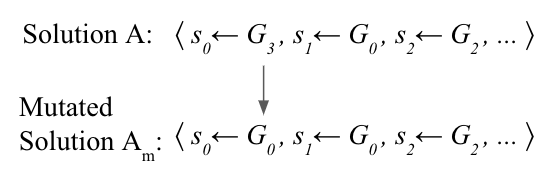
\includegraphics{images/mutation_g.png}
    \caption{An example of a mutation of a solution $A$.}
    \label{fig:mutation_ex}
\end{figure}

\subsection{Crossover}
\label{section:crossover_operator}

The crossover operator is meant to add convergence to already good solutions, so their offspring can reach a local minimum. The crossover used in this work is the k-point crossover~\cite{nomura1997analysis}, which puts a random number of crossover points to indicate where the solution will be split in two parts and have these parts recombined with another solution. An example of this can be seen in Figure~\ref{fig:crossover_ex}, where a crossover point is present in the middle. In terms of this research, it means that a portion of the students will remain in the group defined by their parent solution and the rest will come from another parent solution. Hence, good solutions can explore part of their good results with their children, but at the same time improve their quality if they land with a similar part of another group.\\

\begin{figure*}[!htp]
    \centering
    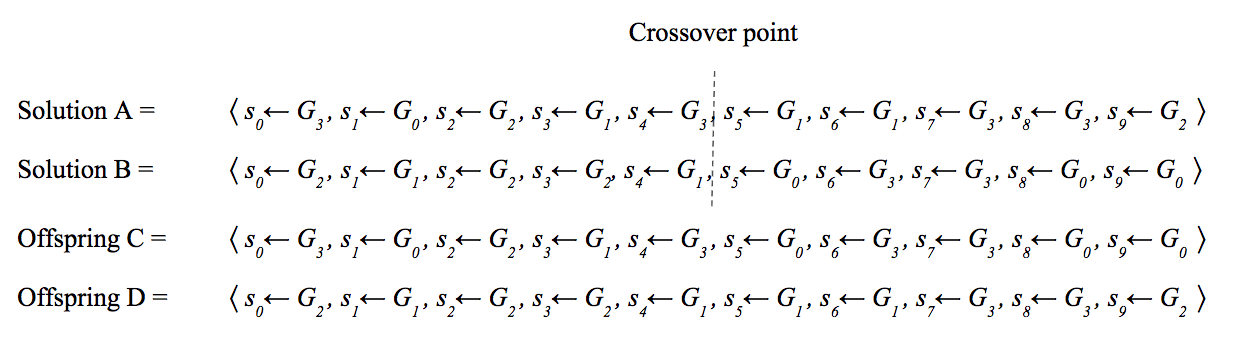
\includegraphics[width=1.0\textwidth]{images/cross_over_g.png}
    \caption{Example of a crossover operation.}
    \label{fig:crossover_ex}
\end{figure*}

It should be noted that, since the assignment is not done with only compatible groups, it is possible that some groups become infeasible. That means that crossover can lead to groups with more students than $gs_{max}$ or less than $gs_{min}$. To prevent this issue, after the crossover operator is applied a repair of the offspring solutions is performed. The whole process can be seen in Algorithm~\ref{alg:crossover}.\\

\begin{algorithm}[H]
    \caption{K-point Crossover}
    \label{alg:crossover}
    \SetAlgoLined 
Select two parents $A$ and $B$ from a parent pool\;\\
Create two offspring $C$ and $D$ a follows:\;\\
Randomly choose $k$ crossover points $cp_1,...cp_k \in {1,...,n-1}$\;\\
\For{$i \gets 1$ to $cp_1$}{
    $c_i \gets a_i$\;\\
    $d_i \gets b_i$
}
$switch \gets 0$
\For{$j \gets 2 to k$}{
    \eIf{$switch = 0$}{
        \For{$i \gets cp_{j-1} + 1$ to $cp_j$}{
            $c_i \gets b_i$\;\\
            $d_i \gets a_i$
        }
        $switch \gets 1$        
    }{
        \For{$i \gets cp_{j-1} + 1$ to $cp_j$}{
            $c_i \gets a_i$\;\\
            $d_i \gets b_i$
        }
        $switch \gets 0$        
    }
}
\eIf{$switch = 0$}{
    \For{$i \gets cp_{j-1} + 1$ to $cp_j$}{
        $c_i \gets b_i$\;\\
        $d_i \gets a_i$
    }
}{
    \For{$i \gets cp_{j-1} + 1$ to $cp_j$}{
        $c_i \gets a_i$\;\\
        $d_i \gets b_i$
    }
}
Perform $Repair$ in $C$ and $D$
\end{algorithm}

\subsection{Repair} \label{sec:Repair}

The defined operators can lead to either a group that ends up with a higher number of students than $gs_{max}$ or a smaller number than $gs_{min}$. For this reason, a repair procedure is performed after the initial population and after each crossover.\\

The repair algorithm consists of checking each group size, if the size is higher than $gs_{max}$, then the group is split in half. On the other hand, if the size is lower than $gs_{min}$, then it requires more members to be feasible and is marked as a pending group $P_g$.  Therefore, after a group $G_i$ with $Size(G_i) > gs_{max}$ is found a user from $G_i$ is assigned to $P_g$, and the algorithm continues until all the groups become feasible.
The fill task can be seen in Algorithm~\ref{alg:repair}.\\

\begin{algorithm}[H]
    \caption{Group Repair}
    \label{alg:repair}
    \SetAlgoLined 
    $A_r = ()$\;\\ \Comment{Initialise a vector that will hold the repaired solution}
    $P_g \leftarrow NULL$\;\\
    \For{$ G_i \in A$}{
        \If{$Size(G_i) > 0$}{
            \If{$P_g$ is not $NULL$ $\textbf{AND}$ $Size(P_g) \leq gs_{max}$ $\textbf{AND}$ $Size(P_g) > gs_{min} $}{
                $A_r \gets MergeGroups(P_g,G_i)$\;\\
                $P_g \leftarrow NULL$
            }\;\\
            \If{$Size(G_i) < gs_{min}$}{
                $A_r \leftarrow SplitGroup(G_i)$ \Comment{Split $G_i$ the group in half}
            }\;\\
            \eIf{$Size(G_i) > gs_{max}$}{
                $P_g \leftarrow G_i$ 
            }{
                $A_r \leftarrow G_i$
            }
        }
    }
\end{algorithm}

\section{Discussion for the following chapter}

This chapter showed the different objective functions to optimise and the definition of the operators to be used. In the following chapter is discussed several exploratory experiments that test these functions and operators. In the case of \textit{Interests Similarity Function} and \textit{Participation Style function}, there is a brief experimentation that lead to their definitions.